\chapter{Methodology} % Main chapter title

\label{Chapter4} % Change X to a consecutive number; for referencing this chapter elsewhere, use \ref{ChapterX}

In this study, we had first to obtain the parameters of phenanthrene using an equation for rings for the SAFT-$\gamma$ Mie force field since they were not available on this force field database \cite{ervik2016}. Hence, this chapter is divided into two sections. The first one describes how we parametrized the phenanthrene molecule and the second one explains how we carried out the solvation free energy simulations. 

\section{Phenanthrene Parameterization}\label{parame}

We implemented the two parameterization strategies for molecules with aromatic rings described in Section \ref{parsaft} for phenanthrene. For both of them, only vapor pressure data \cite{pvphen} were used due to the unavailability of saturated liquid density. We did not estimate the attractive exponent, $\lambda _{a}$. Instead, the value of six was given to it due to its high correlation with the repulsive exponent. The parameterization with the ring equation of \citeonline{muller2017} was carried out with the number of segments equal to five and with a geometry such as that in \figref{fig:fen5}, since this level of coarse-graining was also used for a similar molecule (anthracene) in the original paper.
\begin{figure}[th]
	\centering
	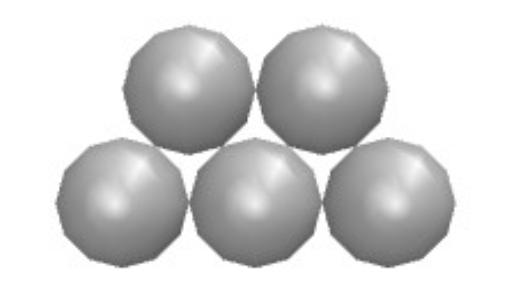
\includegraphics[width=0.25\linewidth]{Figures/fen5}
	\caption{Representation of phenanthrene with the geometry proposed by \citeonline{muller2017}. }
	\label{fig:fen5}
\end{figure}

The minimization was done using the Particle Swarm Optimization (PSO)  method \cite{pso} with the following objective function:
\begin{equation}
\min\limits_{\sigma,\epsilon,\lambda_{r}} F_{obj} = \sum_{i=1}^{N_{p}} \left[\frac{P_{v}^{SAFT}(T_{i},\sigma,\epsilon,\lambda_{r})-P_{v}^{exp}(T_{i})}{P_{v}^{exp}(T_{i})} \right]^2 .
\label{eqn:fobjm}
\end{equation}

Here, $P_{v}^{exp}$ is the experimental vapor pressure and $P_{v}^{SAFT}$ is the vapor pressure obtained with the SAFT-VR Mie EoS. We used the routine proposed by  \citeonline{smithbook} to calculate the bubble point with the EoS. The parameters ($\sigma$, $\epsilon $, and $\lambda _{r}$) from the minimization of the objective function in Eq. \eqref{eqn:fobjm} are the final force field parameters used in molecular simulations. 

The parameterization with the ring equation the \citeonline{lafitte2012} was carried out with $m_{s}=3$, so that every bead would represent one aromatic ring, such as depicted in Fig:

\begin{figure}[th]
	\centering
	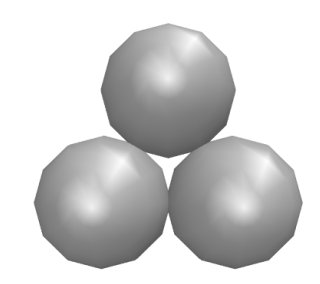
\includegraphics[width=0.15\linewidth]{Figures/fe3}
	\caption{Representation of phenanthrene with the geometry proposed by \citeonline{lafitte2012}.}
	\label{fig:fen3}
\end{figure}

The first part of the estimation followed the same procedure described above for the \citeonline{muller2017} equation. However, as explained in Section \ref{parsaft}, the \citeonline{lafitte2012} equation requires the estimation of correction factors $c_{\sigma}$ and $c_{\epsilon}$ (Eqs. \eqref{eqn:csigma} and \eqref{eqn:ceps}). We then estimated these parameters by using the PSO method with Eq. \eqref{eqn:fobjla}. In this equation, vapor pressures and saturated liquid densities from molecular simulations are required. We then decided to use the Gibbs Ensemble Monte Carlo method on the NVT ensemble, explained in Section \ref{gemc}, to obtain these equilibrium properties at eight different temperatures since this method does not use an explicit interface.

The boxes for the GEMC-NVT simulations were generated by inserting 400 molecules of phenanthrene into one liquid box and 100 molecules of phenanthrene into the other one using the Playmol package \cite{playmol}, which is integrated with the Packmol package \cite{packmol}. Initial densities of each box were made equal to the saturated densities found with the SAFT-VR Mie Eos, aiming at avoiding the migration of all molecules to a single phase during the simulation. The GEMC-NVT simulations were carried using the Cassandra software \cite{doi:10.1063/1.3644939},  which was developed to perform Monte Carlo simulations. The equilibration and production times lasted around  $10^{4}$ and $5 \times 10^{4}$ MC cycles, respectively. Each MC cycle corresponded to $10^3$ rotation trials, $10^3$ translation trials, $10^2$ molecule insertion trials, $10^2$ molecule deletion trials, and 10 volume exchange trials. The cut-off distance was equal to $20$ \AA  $\,$ and we did not use long-range interactions. The saturated vapor density ($\rho_{vap}$), the saturated liquid density ($\rho_{liq}$), and the vapor pressure ($P_{v}$) were sampled at each 100 MC cycles. Later on, these data were divided into five blocks for calculation of their averages and standard deviations. With the correction factors found after the estimation with the simulation data, we calculated with Eqs. \eqref{eqn:simsigma} and \eqref{eqn:simeps} the $\sigma$ and $\epsilon$ parameters. \citeonline{lafitte2012} proposes that are the final parameters to be used in molecular simulation. Hence, an iterative simulation is not required, and the set of optimal parameters can be obtained with one group of molecular simulations. 

\section{Solvation Free Energy Simulations}\label{solvme}

Using the parameters for phenanthrene estimated with the \citeonline{muller2017} approach and the SAFT-$\gamma$ Mie force field parameters available for other compounds, we carried out molecular dynamics simulations to estimate solvation free energy differences. The chosen software package to perform the simulations was the LAMMPS  \cite{lammps}. In this package, the equations of motion were integrated with the velocity-Verlet algorithm \cite{verlet} with a time step of 2 fs. As required by the coarse-grained model,  molecules with more than one bead were treated as rigid bodies. The thermostat and the barostat were the Nos\'{e} Hoover chains as described originally in \citeonline{PhysRevA.31.1695}, \citeonline{doi:10.1063/1.463940}, and \citeonline{doi:10.1063/1.467468} with damping factors of 100 and 1000 time steps, respectively. For the rigid bodies in our simulations, we used the rigid-body algorithm of \citeonline{kamberaj}. Electrostatics interactions are not explicitly accounted for the SAFT-$\gamma$ Mie force field. Hence, we did not compute Coulombic interactions. The potential cutoff was equal to 20 \AA $\,$ \cite{muller2017} with a neighbor list skin of 2 \AA. The initial configurations of the solvated systems were also generated using the Playmol package, which is integrated with the Packmol package. For the binary mixtures, one molecule of solute and a varying number of solvent molecules- 700 molecules of toluene, 700 molecules of octanol, 1024 molecules of hexane, 3000 molecules of water - were randomly added to a cubic box. Besides the systems with pure substances acting as solvents, we performed simulations to study solvation free energy of phenanthrene in a mixture of toluene and carbon dioxide with different weight fractions ($w_{CO_{2}}$). The  system consisted of one molecule of phenanthrene for all the cases and 123 molecules of $CO_{2}$ and 618 molecules of toluene ($w_{CO_{2}} = 0.087$); 166 molecules of $CO_{2}$ and 589 molecules of toluene ($w_{CO_{2}} = 0.119$); 232 molecules of $CO_{2}$ and 545 molecules of toluene ($w_{CO_{2}} = 0.169)$; 380 molecules of $CO_{2}$ and 446 molecules of toluene ($w_{CO_{2}} = 0.289$). The substances used in this study were selected with the intention of testing the force field with standard sets used as a benchmark in solvation free energy calculations, with aromatic substances used as models to asphaltenes and with water, which probably is the most used solvent in computational studies.

All simulations were performed with the constant temperature and pressure values of 298 K and 1 bar, except the ones containing carbon dioxide. These had the temperature of 298 K and the pressure of the experimental liquid-phase equilibrium correspondent to each composition of the system $CO_{2}+$toluene \cite{co2toliq}. For all simulations, the initial box was equilibrated at the NPT ensemble for 2 ns, and the resulting configurations were used as the initial configuration of the expanded ensemble simulations. These were carried out with the LAMMPS user package for expanded ensemble simulations with the Mie Potential developed by our research group, available at https://github.com/atoms-ufrj/USER-ALCHEMICAL. 

During these expanded ensemble simulations, the sampling of a new alchemical state was tried at every 10 MD steps. To define the optimal values of $\lambda$ and $\eta$ corresponding to each state, trial simulations, having around 9 ns of production time, were carried out. In the first simulation, we chose the group of $\lambda$ values arbitrarily, and we either set all $\eta 's$ to zero or assigned values previously found for similar solute-solvent pairs. The subsequent group of $\eta 's$ were estimated with the flat histogram approach (Eq. \eqref{eqn:weight}). We then did another trial simulation with the new weights. The results of this simulation were used to optimize the group of $\lambda 's$ by minimizing the number of round trips, as described in Section \ref{ee}. The $\eta 's$ corresponding to the newest group of $\lambda 's$ were interpolated linearly from the free energy differences. With the final values of $\eta$ and $\lambda $ defined for each mixture, larger simulations with a production time of 20 ns were carried out. 

Since the employed force field considers that the beads do not have charges, there are no Coulombic interactions and the $\Delta G$ in Eq. \eqref{eq:freesolv} becomes equal to $\Delta G_{3 \rightarrow 4} $. The post-processing method used to effectively calculate free energy differences with the potential energies obtained from the expanded ensemble simulations was the Multistate Bennett Acceptance Ratio (MBAR) method, described in Section \ref{mbar}. The software alchemical-analysis \cite{klimovich} was utilized to obtain the $\Delta G_{solv}$ with MBAR and to assess the quality of the results. After the first estimations, we realized that the binary interaction parameter of Eq. \eqref{eqn:epsmix} was necessary for systems containing water. Hence, we estimated  $k_{ij}$ for these pairs and, for all the other pairs, we set  $k_{ij}$ to zero. The estimation was done by performing trial expanded ensemble simulations in three values of $k_{ij}$, as suggested by \citeonline{ervik20162}. With the $\Delta G_{solv}$ obtained with these simulations, we did a linear fit to obtain the refined value of the parameter. We used this strategy because the estimation with SAFT VR Mie EoS gave poor results for the solvation free energies.

